\documentclass[12pt]{article}

\usepackage[utf8]{inputenc}
\usepackage{color, colortbl}
\usepackage{amsmath}
\usepackage{graphicx}


\graphicspath{ {./images/} }
\definecolor{Gray}{gray}{0.9}



\mathcode`*=\string"8000
\begingroup
\catcode`*=\active
\xdef*{\noexpand\textup{\string*}}
\endgroup
\renewcommand{\baselinestretch}{1.5}
\title{NFA a DFA.}
\author{Luis Diego Jiménez Delgado\\ 2CM5}
\date{24 de septiembre del 2019}

\begin{document}
    \maketitle
    \newpage
 
    { \large \tableofcontents }
    \newpage
    \section{Automata de Ajedrez}
        Considerando el automata NFA de la propesuta de los reyes debemos de obtener el diagrama DFA de este mismo para esto observar lo siguiente.
        \begin{center}
            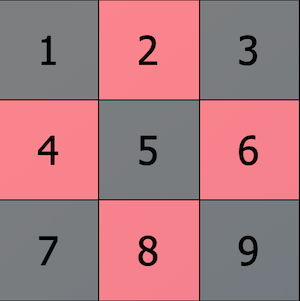
\includegraphics{table}
         \end{center}
         Podemos desarrollar la siguiente tabla de entradas, desarrollamos lo siguiente para ver los pasos que debemos desarrollar.
         \begin{center}
            \newcolumntype{g}{>{\columncolor{Gray}}c}
            \begin{table}[ht]
                \centering
                \begin{tabular}{c|g|c}
                \hline
                    &r &b\\
                \hline
                1&2,4&5\\
                2&4,6&1,3,5\\
                3&2,6&5\\
                4&2,8&1,5,7\\
                5&2,4,6,8&1,3,7,9\\
                6&2,8&3,5,9\\
                7&4,8&5\\
                8&4,6&5,7,9\\
                9&6,8&5\\
            \end{tabular}
            \end{table}
        \end{center}
     	Después de analizar los datos del de la tabla de transiciones \\
       
        \begin{center}
            \newcolumntype{g}{>{\columncolor{Gray}}c}
            \begin{table}[ht]
                \centering
                \begin{tabular}{c|c|c}
                    &r &b\\
               	\hline
                	--- $>$\{1\}&\{2,4\}&\{5\}\\
           	 \end{tabular}
            \end{table}
            Evaluando:
            \begin{table}[ht]
                \centering
                \begin{tabular}{c|c|c}
                    &r &b\\
               	\hline
                	--- $>$\{1\}&\{2,4\}&\{5\}\\
		\{2,4\}&\{2,4,6,8\}&\{1,3,5.7\}\\
		\{5\}&\{2,4,6,8\}&\{1,3,7,9\}\\
		\{2,4,6,8\}&\{2,4,6,8\}&\{1,3,5,7,9\}\\
		\{1,3,5,7\}&\{2,4,6,8\}&\{1,3,5,7,9\}\\
		$ *$\{1,3,7,9\}&\{2,4,6,8\}&\{5\}\\
		$ *$\{1,3,5,7,9\}&\{2,4,6,8\}&\{1,3,5,7,9\}\\
           	 \end{tabular}
            \end{table}
            
        \end{center}
        Después de haber desarrollado la tabla de subconjuntos encontramos lo siguiente para la construcción del mismo, es importante considerar que este se intuye de las soluciones que obtuvimos:
        \begin{center}
              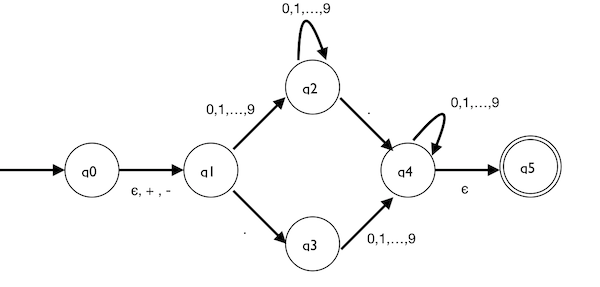
\includegraphics{dia1}
        \end{center}
        
        
        \newpage
    \section{Automata de decimales}
	Se debe de construir el DFA del NFA de un autómata que es capaz de detectar número decimales, es complejo decir exactamente el funcionamiento del automata sin hacer referencia al diagrama de este.        
	 \begin{center}
            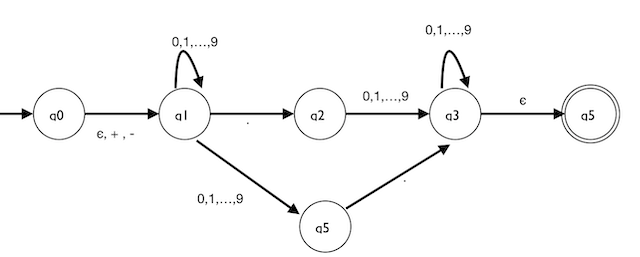
\includegraphics{dia2}
         \end{center}                                           
         Debemos de considerar que es importante eliminar a la cadena vacía del autómata para que se pueda simplificar un poco que de alguna u otra manera. 
         \begin{center}
              \newcolumntype{g}{>{\columncolor{Gray}}c}
          	 \begin{table}[ht]
                 \centering
                \begin{tabular}{c|c|c|c|c}
                    && $\epsilon$, +, -& 0,1,...,9  &.\\
               	\hline
		A&\{q0\}&\{q1\}&\{\}&\{\}\\
		B&\{q1\}&\{\}&\{q1,q4\}&\{q2\}\\
		C&\{q1,q4\}&\{\}&\{q1,q4\}&\{q3\}\\
		D&\{q2\}&\{\}&\{q3\}&\{\}\\
		E&\{q3\}&\{q5\}&\{q3\}&\{\}\\
		F&\{q5\}&\{\}&\{\}&\{\}\\
           	 \end{tabular}
            \end{table}
         \end{center}
          \begin{center}
            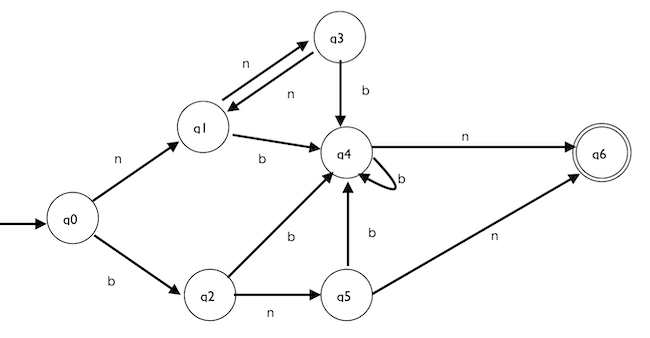
\includegraphics{diar2}
         \end{center}   
\end{document}